\chapter{Vector Basics}
    \section{Recommended Texts}
        The following books are recommended for the course. The first one will be followed by the instructor.
        \begin{enumerate}
            \item Engineering Electromagnetics 8th Edition by John Buck \& William H. Hayt
            \item Electromagnetics John D. Kraus
            \item Introduction to Electrodynamics by David J. Griffiths
            \item Classical Electrodynamics by John David Jackson
        \end{enumerate}
    \section{What is a Vector?}
        From a mathematical standpoint a vector is an element of a vector space. From a physical point of view a vector is a quantity that requires a magnitude as well as a direction to be represented.
    \section{Unit vectors in Rectangular Coordinate System}
        In a Rectangular Coordinate System (RCS), a vector can be represented as a linear sum of three unit vectors, namely $\vec{a}_x$, $\vec{a}_y$ and $\vec{a}_z$. In case of two dimensions, $\vec{a}_z$ is not needed. This is also depicted in figure~\ref{fig:vectors}.
        \begin{figure}
            \centering
            \subfloat[A vector in two dimensions]{
                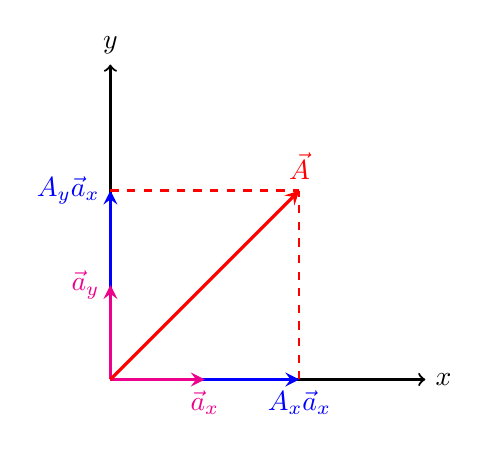
\begin{tikzpicture}
    [scale=4,
    axis/.style={->,thick},
    vector/.style={-stealth,very thick},
    vector guide/.style={dashed,red,thick}]

    \coordinate (O) at (0, 0);
    \def\u{0.3}
    \def\v{0.6}

    % drawing axes
    \draw[axis] (O) -- (1, 0) node[anchor=west]{$x$};
    \draw[axis] (O) -- (0, 1) node[anchor=south]{$y$};

    % drawing the vector's components
    \draw[vector, blue] (O) -- (\v, 0) node[anchor=north]{$A_x\vec{a}_x$};
    \draw[vector, blue] (O) -- (0, \v) node[anchor=east]{$A_y\vec{a}_x$};

    % drawing unit vectors
    \draw[vector, magenta] (O) -- (\u, 0) node[anchor=north]{$\vec{a}_x$};
    \draw[vector, magenta] (O) -- (0, \u) node[anchor=east]{$\vec{a}_y$};

    % drawing vector A
    \draw[vector, red] (O) -- (\v, \v) node[anchor=south]{$\vec{A}$};

    % drawing vector guides
    \draw[vector guide] (\v, 0) -- (\v, \v);
    \draw[vector guide] (0, \v) -- (\v, \v);

\end{tikzpicture}
            }
            \subfloat[A vector in three dimensions]{
                % sets up the perspective from which we are looking at the picture {theta}{phi}
% {theta} defines the rotion by x axis while {phi} defines the rotation by z axis
\tdplotsetmaincoords{60}{120}

\begin{tikzpicture}
    [scale=4,
    tdplot_main_coords,
    axis/.style={->,black,thick},
    vector/.style={-stealth,very thick},
    vector guide/.style={dashed,red,thick}]

    \coordinate (O) at (0, 0, 0);

    % this should serve as our unit vector
    \def\u{0.3} 
    \def\v{0.6}
    % drawing axes
    \draw[axis] (0, 0, 0) -- (1, 0, 0) node[anchor=north east]{$x$};
    \draw[axis] (0, 0, 0) -- (0, 1, 0) node[anchor=north west]{$y$};
    \draw[axis] (0, 0, 0) -- (0, 0, 1) node[anchor=south]{$z$};

    % drawing the components of the vector A: Drawing them first so the unit vectors do appear
    \draw[vector, blue] (O) -- (\v, 0, 0) node[anchor=south east]{$B_x\vec{a}_x$};
    \draw[vector, blue] (O) -- (0, \v, 0) node[anchor=south west]{$B_y\vec{a}_y$};
    \draw[vector, blue] (O) -- (0, 0, \v) node[anchor=south east]{$B_z\vec{a}_z$};

    % drawing the unit vectors
    \draw[vector, magenta] (O) -- (\u, 0, 0) node[anchor=south east]{$\vec{a}_x$};
    \draw[vector, magenta] (O) -- (0, \u, 0) node[anchor=south west]{$\vec{a}_y$};
    \draw[vector, magenta] (O) -- (0, 0, \u) node[anchor=east]{$\vec{a}_z$};

    % drawing the main vector B
    \draw[vector, red] (O) -- (\v, \v, \v) node[anchor=south east]{$\vec{B}$};

    % projection on xy axis
    \draw[vector guide] (\v, 0, 0) -- (\v, \v, 0);
    \draw[vector guide] (0, \v, 0) -- (\v, \v, 0);
    \draw [vector guide] (\v, \v, 0) -- (\v, \v, \v);

    % drawing projection on yz axis
    \draw[vector guide] (0, \v, 0) -- (0, \v, \v);
    \draw[vector guide] (0, 0, \v) -- (0, \v, \v);
    \draw[vector guide] (0, \v, \v) -- (\v, \v, \v);

    % drawing projection on xz axis
    \draw[vector guide] (0, 0, \v) -- (\v, 0, \v);
    \draw[vector guide] (\v, 0, 0) -- (\v, 0, \v);
    \draw[vector guide] (\v, 0, \v) -- (\v, \v, \v);


\end{tikzpicture}
            }
            \caption{}
            \label{fig:vectors}
        \end{figure}
    \section{Dot Product}
        Suppose we have two vectors $\vec{A}$ and $\vec{B}$. $\vec{A}$ can be represented as:
        $$\vec{A} = A_x\vec{a}_x + A_y\vec{a}_y + A_z\vec{a}_z$$
        Similarly, $\vec{B}$ can be represented as:
        $$\vec{B} = B_x\vec{a}_x + B_y\vec{a}_y + B_z\vec{a}_z$$
        Their dot product, $\vec{A}\cdot \vec{B}$, which is a scalar quantity, is defined as:
        $$\vec{A}\cdot \vec{B} = |\vec{A}||\vec{B}|\cos \theta$$
        In case when $\theta$ becomes $90^{\circ}$ the dot product automatically reduces to zero. Thus one can easily conclude that the dot product of two perpendicular vectors shall always be zero. This makes expressing the dot product in terms of its components pretty straight forward.
        $$\vec{A}\cdot \vec{B} = \left(A_x\vec{a}_x + A_y\vec{a}_y + A_z\vec{a}_z\right)\cdot \left(B_x\vec{a}_x + B_y\vec{a}_y + B_z\vec{a}_z\right)$$
        \begin{equation}\label{eq:dotproduct}
           \vec{A}\cdot \vec{B} = A_xB_x + A_yB_y + A_zB_z
        \end{equation}
        A vector can also be represented in the form of column vector as:
        $$ \vec{A} = \begin{bmatrix}A_x \\A_y \\A_z\\ \end{bmatrix} \quad \vec{B} = \begin{bmatrix}B_x \\B_y \\B_z\\ \end{bmatrix} $$
        In that case the dot product, also called inner product in this context, is defined as:
        $$ \mathbf{A}^{T}\mathbf{B} $$
        If the vectors $\vec{A}$ and $\vec{B}$ are of the order $n \times 1$ their inner product will have the order $ 1 \times \left(n \times n\right) \times 1 = 1 \times 1$. Thus the result will be a scalar quantity.
        The opposite of the inner product is known as the outer product also called the cross product which we will get to in a later topic.
        
        